\documentclass[12pt,a4paper]{article}
\usepackage{blindtext}
\usepackage{graphicx}
\usepackage[utf8]{inputenc}
\usepackage[margin=0.65in]{geometry}
\usepackage{multicol}
\usepackage{wrapfig}
\usepackage[dvipsnames]{xcolor}
\usepackage{framed}
\usepackage[most]{tcolorbox}
\usepackage{pgfgantt}
\usepackage{tikz}
\usetikzlibrary{arrows.meta}
\usepackage[dvipsnames]{xcolor}
\definecolor{aliceblue}{rgb}{0.94, 0.97, 1.0}
\colorlet{shadecolor}{aliceblue}
\setlength\parindent{0pt}
\usepackage{charter}
\usepackage{environ}
\usepackage{tikz}
\usetikzlibrary{calc,matrix}
\usetikzlibrary{positioning,fit,calc}
\usepackage{float}
\usepackage{url}
% code by Andrew:
% http://tex.stackexchange.com/a/28452/13304
\makeatletter
\let\matamp=&
\catcode`\&=13
\makeatletter
\def&{\iftikz@is@matrix
	\pgfmatrixnextcell
	\else
	\matamp
	\fi}
\makeatother

\newcounter{lines}
\def\endlr{\stepcounter{lines}\\}

\title{COMPSCI 702 - Security for Smart-devices}
\date{Semester 1, 2018}
\begin{document}
\maketitle
\tableofcontents{}

\section*{Disclaimer}
\textit{This study guide is based off the lecture slides prepared for CS702. It is provided as-is and may contain errors, though effort has been made to minimize this. This resource is not exhaustive and may not contain additional content not covered by the slides.}
\newpage

\section{Access Control}
\subsection{Security objectives}
\begin{shaded}
\begin{itemize}
	\item \textbf{Confidentiality.} Protection of the data.
	\item \textbf{Integrity.} Ensure data is not altered by unauthorized parties.
	\item \textbf{Availability.} Ensure timely access to data.
	\item \textbf{Authentication.} Identify whether communicating entity is who it claims to be.
	\item \textbf{Authorization.} Regulate access to data.
\end{itemize}
\end{shaded}
\subsection{Access control requirements}
The inputs need to be \textit{reliable}, with authenticated entities or genuine information. The \textbf{principle of least privileges} grants the minimum set of access rights to do a job. Furthermore, only a special entity (administrator) can manage (grant/revoke/update) access rights.
\subsection{Elements of access control}
\begin{shaded}
\begin{itemize}
	\item \textbf{Subject.} An entity that can access objects. It can be a user or a process representing a user or an application.
	\item \textbf{Object.} An entity (file, directory, resource) that needs to be protected.
	\item \textbf{Access right.} An access right $r \in R$ describes how a subject $s \in S$ can access an object $o \in O$. Examples include: read, write, execute, create, delete, search, etc.
	\item \textbf{Access control function $f(s, o, r)$} looks up the access right $r$ for combination $(s, o)$. It grants access on a successful match.
	\item \textbf{Security administrator.} Entity that manages access rights.
	\item \textbf{Auditor.} Entity that inspects whole authorization system.
\end{itemize}	
\end{shaded}
\subsection{Access control models}
There are 5 main models for access control:
\begin{itemize}
	\item Discretionary access control (DAC),
	\item Mandatory access control (MAC),
	\item Role-based access control (RBAC),
	\item Usage control (UCON), and
	\item Policy-based access control (PBAC).
\end{itemize}
\subsubsection{Discretionary access control}
Users can protect what they own. The owner can grant access to subjects. Access is granted based on the identity of the requester. These mechanisms are adequate for honest users, but are vulnerable to Trojan horses.\\

DAC is used in operating systems and DBMS. An example is Linux file permissions: \texttt{rwxr-x--x}.

\subsubsection*{Access control matrix}
\begin{shaded}
\begin{center}
\begin{tabular}{lllll}
                            & File 1                                                                            & File 2                                                                            & File 3                                                                            & File 4                                                                          \\ \cline{2-5} 
\multicolumn{1}{l|}{User A} & \multicolumn{1}{l|}{\begin{tabular}[c]{@{}l@{}}owner\\ read\\ write\end{tabular}} & \multicolumn{1}{l|}{}                                                             & \multicolumn{1}{l|}{\begin{tabular}[c]{@{}l@{}}owner\\ read\\ write\end{tabular}} & \multicolumn{1}{l|}{}                                                           \\ \cline{2-5} 
\multicolumn{1}{l|}{User B} & \multicolumn{1}{l|}{read}                                                         & \multicolumn{1}{l|}{\begin{tabular}[c]{@{}l@{}}owner\\ read\\ write\end{tabular}} & \multicolumn{1}{l|}{write}                                                        & \multicolumn{1}{l|}{read}                                                       \\ \cline{2-5} 
\multicolumn{1}{l|}{User C} & \multicolumn{1}{l|}{\begin{tabular}[c]{@{}l@{}}read\\ write\end{tabular}}         & \multicolumn{1}{l|}{read}                                                         & \multicolumn{1}{l|}{}                                                             & \multicolumn{1}{l|}{\begin{tabular}[c]{@{}l@{}}own\\ read\\ write\end{tabular}} \\ \cline{2-5} 
\end{tabular}
\end{center}
An \textbf{access control list}	is a list of access rights on an object. A \textbf{capability list} refers to a user's permissions on different objects. In the diagram, columns are ACLs and rows are capability lists.
\end{shaded}
\subsubsection{Mandatory access control}
MAC restricts access on the basis of security labels. Entities cannot enable other entities to access their resources. Users have security clearance, and resources have security labels that contain data classification.\\

This model is used when information classification and confidentiality are very important, such as in the military. The \textbf{Bell-LaPadula model} (BLP) is used in the US Department of Defence. The \textbf{Biba model} is implemented in the FreeBSD MAC policy. A combined version is used in Android.

\subsubsection*{Bell-LaPadula model}
Goal: Control \textbf{confidentiality of information}.
\begin{itemize}
	\item \textbf{Simple security property.} No read up.
	\item \textbf{*(Star)property.} No write down.
	\item \textbf{Strong *(star)property} No write down and no write up.
\end{itemize}

\subsubsection*{Biba integrity model}
Goal: Control \textbf{integrity of information}.
\begin{itemize}
	\item \textbf{Simple integrity axiom.} No read down.
	\item \textbf{*(Star)-integrity axiom.} No write up.
\end{itemize}
\subsubsection{Role-based access control}
RBAC maps roles to access rights. Supports complex access control. Reduces administrative errors. Flexible to move users or permissions in/out of roles. Least privilege; restrict access according to needs.

\subsubsection*{RBAC model}
\begin{shaded}
\begin{itemize}
	\item \textbf{User.} A human being. Usually. They are assigned roles (\textbf{user assignment, UA}).
	\item \textbf{Permissions.} Approval of a mode of access to some object. They represent what operations could be performed on objects.
	\item \textbf{Roles.} Job title. Roles are assigned permissions (\textbf{permission assignment, PA}).
	\item \textbf{Assignments.} User-role and role-permission.
	\item \textbf{Session.} Mapping between user and an activated subset of assigned roles.
	\item \textbf{Constraints.} Constraintsd are present on sessions, assignments, and roles.
\end{itemize}	
\end{shaded}

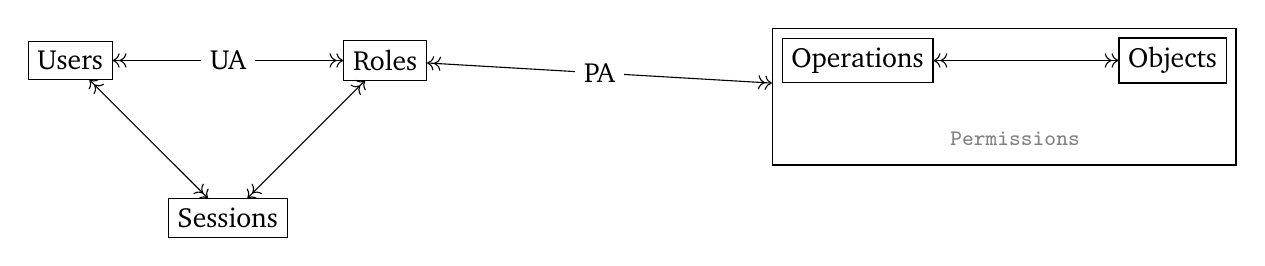
\begin{tikzpicture}[title/.style={font=\fontsize{8}{8}\color{black!50}\ttfamily}]
\node (h) at (12, 1) [title] {Permissions};
\node (a) at (0, 2) [rectangle, draw] {Users};
\node (b) at (4, 2) [rectangle, draw] {Roles};
\node (c) at (2, 0) [rectangle, draw] {Sessions};
\node (d) at (10, 2) [rectangle, draw] {Operations};
\node (e) at (14, 2) [rectangle, draw] {Objects};
\node (f) at (8, 2) [rectangle, draw, fit={(h) (d) (e)}] {};
\draw [<<->>] (a) -- (b) node [midway, fill=white] {UA};
\draw [<<->>] (a) -- (c);
\draw [<<->>] (b) -- (c);
\draw [<<->>] (b) -- (f) node [midway, fill=white] {PA};
\draw [<<->>] (d) -- (e);
\end{tikzpicture}

\subsubsection*{Controlling usage of resources}
DAC, MAC, and RBAC are concerned with checking access rights of entities. Once the access is granted, no more control is enforced.

\subsubsection{Usage control}
UCON doesn't just regulate access to an object, but also focuses on controlling usage. Addresses DRM. DAC, MAC, and RBAC can be expressed by UCON.

\subsubsection*{UCON model}
\begin{shaded}
\begin{itemize}
	\item \textbf{Subjects.} Entities that perform actions.
	\item \textbf{Objects.} Entities accessed by subjects.
	\item \textbf{Rights.} Set of actions.
	\item \textbf{Authorization.} Functional predicates that have to be evaluated for usage decision.
	\item \textbf{Obligations.} Functional predicates that verify mandatory requirements that must have been performed by subject.
	\item \textbf{Conditions.} Environmental/system based decision factors (time, status, etc.)
\end{itemize}	
\end{shaded}
\subsubsection{Policy-based access control}
In PBAC, an authorization policy governs access rights of subjects over objects. Policies are specified independently of entities. This provides a coherent view of access control in a system, and a separation between AC logic and enforcement mechanism.\\

An approach is XACML.

\subsubsection*{PBAC entities}
\begin{itemize}
	\item \textbf{Policy administrator.} Administrates access policies.
	\item \textbf{Policy administration point (PAP).} Interface for policy administration.
	\item \textbf{Policy store.} Repository to store policies.
	\item \textbf{Subject.} Entity that makes access requests.
	\item \textbf{Resources.} Target objects requested by subject.
	\item \textbf{Policy enforcement point (PEP).} Enforces access policies and grants access to resources.
	\item \textbf{Policy decision point (PDP).} Evaluates access policies.
	\item \textbf{Policy information point (PIP).} Provides contextual information.
\end{itemize}
\section{Android Security}
\subsection{Introduction to Android}
Android is a smartphone (open-source) OS currently developed by Google based on the Linux kernel. The SDK was released in November 2007 for Java, followed by the NDK (native development kit) in June 2009 for C and C++. The \textbf{Open Handset Alliance} is a consortium of 84 firms for developing open standards for mobile devices.\\

Android \textbf{fragmentation} is a problem. Vendors can customize the OS for their own devices by including their own apps. Some of these apps may compromise security/privacy as they have technical vulnerabilities. Vendors also might not push updates as frequently, and leave devices a few versions behind. Some vendors stop supporting their devices afterwards as well. \textit{The lack of support can lead to vulnerabilities.}\\

Android is considered \textbf{middleware} between the Linux kernel and its set of APIs. Android apps are mainly written in Java, and only Android apps can run on Android devices. Through the APIs, apps can access device information/components.

\includegraphics[width=\textwidth]{graphics/androidanatomy}

\paragraph{Linux kernel}
Android is built on the Linux kernel\footnote{It is \textbf{not} Linux.}. There is no \texttt{glibc} support, nor does it include the full set of Linux utilities. There are some kernel enhancements.\\

The Linux kernel was chosen as it has great memory/process management. It also has a permissions-based security model, a proven driver model, support for shared libraries. The Linux kernel is also open-source.

\paragraph{Binder}
Applications and services may run in separate processes but must communicate and share data. \textbf{Issue:} Inter-process communication (IPC) can introduce significant processing overhead and security holes. \textbf{Solution:} Driver to facilitate IPC.

\paragraph{Power management}
Mobile devices run on battery power with limited capacity. The power management features are built on top of Linux power management, but has more aggressive power management policy.

\subsubsection*{Native libraries}
Bionic \texttt{libc} is a custom \texttt{libc} implementation.\\

Why Bionic? \texttt{glibc} is licensed under LGPL, which prevents static linking of proprietary software. The size needs to be small as it will load in each process, and needs to be efficiency due to limited CPU power. \textbf{Bionic \texttt{libc}} is under the BSD license, is small, and efficient due to a custom pthread implementation. It does not support some POSIX features, is not compatible with \texttt{glibc}, and all native code must be compiled against Bionic.

\subsubsection*{Hardware abstraction layer}
This layer is a user-space C/C++ layer which separates the Android platform logic from the hardware interface.\\

A user-space HAL is necessary as 1) not all components have standardized kernel driver interfaces; 2) kernel drivers are licensed under GPL, which exposes any proprietary IP; and 3) Android has specific requirements for hardware drivers.

\subsubsection*{Android runtime}
\paragraph{Dalvik VM}
Android's custom clean room implementation. Provides application portability and runtime consistency. This runs Dalvik bytecode (optimized file format \texttt{.dex}). Java \texttt{.class}/\texttt{.jar} files are converted to \texttt{.dex} at build time.\\

The VM is also designed for embedded environment. It supports multiple virtual machine processes per device. It has a highly CPU-optimized bytecode interpreter, and uses runtime memory very efficiently.

\paragraph{Core libraries}
These are Core APIs for Java which provide a powerful and simple/familiar development platform. They are basically Java wrappers around C/C++ based libraries.

\subsubsection*{Application framework}
These are services essential for Android. Apps don't access them directly.

\subsubsection*{Applications}
These are applications.

\subsubsection{Runtime}
At startup, the bootloader loads the Linux kernel and starts the \texttt{init} process. The \texttt{init} process starts the \textbf{zygote} process, a nascent process that initializes a Dalvik VM instance. It forks on request to create VM instances for managed processes. It uses copy-on-write to maximize re-use and minimize footprint. \textit{There is an instance of DalvikVM per APK.}\\

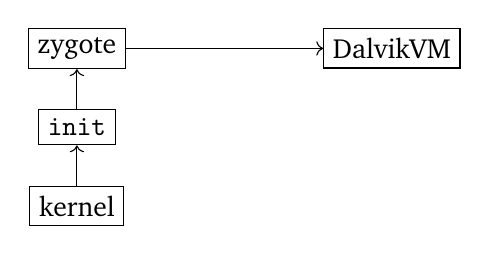
\begin{tikzpicture}[title/.style={font=\fontsize{8}{8}\color{black!50}\ttfamily}]
\node (a) at (0, 0) [rectangle, draw] {kernel};
\node (b) at (0, 1) [rectangle, draw] {\texttt{init}};
\node (c) at (0, 2) [rectangle, draw] {zygote};
\node (d) at (4, 2) [rectangle, draw] {DalvikVM};

\draw [->] (a) -- (b) node [midway] {};
\draw [->] (b) -- (c) node [midway] {};
\draw [->] (c) -- (d) node [midway] {};

\end{tikzpicture}

\includegraphics[width=\textwidth]{graphics/androidrt}

\subsubsection*{Android security objectives}
The goals are to protect user data, protect system resources (+network), and provide application isolation. 

\begin{shaded}
\textbf{Key Android security features:}
\begin{itemize}
	\item Robust security at OS level through Linux kernel
	\item Mandatory app sandboxing for all applications
	\item Secure IPC
	\item Application signing
	\item Application-defined and user-granted permissions
\end{itemize}	
\end{shaded}

\subsection{Android application model}
\section{iOS Security}
\section{Seminars}




\end{document}
